\documentclass{sig-alternative}
% \documentclass[conference]{IEEEtran}
\usepackage{color}
\usepackage{listings}
\usepackage{graphicx} 
\usepackage{multirow}
\usepackage[table,xcdraw]{xcolor}
\usepackage{cite}
\usepackage{paralist}
\usepackage[table,xcdraw]{xcolor}
\usepackage{siunitx}
\usepackage{rotating}
\usepackage{eqparbox}


\usepackage[framemethod=tikz]{mdframed}
\usepackage{lipsum}
\usetikzlibrary{shadows}
\newmdenv[tikzsetting= {fill=white!20},roundcorner=10pt, shadow=true]{myshadowbox}




\usepackage{graphics}
\usepackage{colortbl} 
\usepackage{multirow}
\usepackage{times}
\usepackage{balance}
\usepackage{picture}
% \usepackage{multirow}
\usepackage[table,xcdraw]{xcolor}
\usepackage{soul}

\usepackage{fourier} 
\usepackage{array}
\usepackage{makecell}

\renewcommand\theadalign{cb}
\renewcommand\theadfont{\bfseries}
\renewcommand\theadgape{\Gape[4pt]}
\renewcommand\cellgape{\Gape[4pt]}

\usepackage{verbatim}
\usepackage{algorithm}
\usepackage{algorithmicx}
\usepackage{algpseudocode}
\usepackage[export]{adjustbox}
\renewcommand{\footnotesize}{\scriptsize}
\definecolor{lightgray}{gray}{0.8}
\definecolor{darkgray}{gray}{0.6}
\renewcommand{\algorithmicrequire}{\textbf{Input:}}
\renewcommand{\algorithmicensure}{\textbf{Output:}}
\usepackage[table]{xcolor}
\definecolor{Gray}{rgb}{0.88,1,1}
\definecolor{Gray}{gray}{0.85}
\definecolor{Blue}{RGB}{0,29,193}
\newcommand{\G}{\cellcolor{green}}
\newcommand{\Y}{\cellcolor{yellow}}


\definecolor{MyDarkBlue}{rgb}{0,0.08,0.45} 
\lstset{
    language=Python,
    basicstyle=\ttfamily\fontsize{2.7mm}{0.8em}\selectfont,
    breaklines=true,
    prebreak=\raisebox{0ex}[0ex][0ex]{\ensuremath{\hookleftarrow}},
    frame=l,
    showtabs=false,
    showspaces=false,
    showstringspaces=false,
    keywordstyle=\bfseries,
    emph={furthest,gale,better,improved,where,fastmap,split,project,mutate,mutate1}, emphstyle=\bfseries\color{blue},
    stringstyle=\color{green!50!black},
    commentstyle=\color{gray}\itshape,
    numbers=left,
    captionpos=t,
    escapeinside={\%*}{*)}
}


%%% graph
\newcommand{\crule}[3][darkgray]{\textcolor{#1}{\rule{#2}{#3}}}
%\newcommand{\rone}{\crule{1mm}{1.95mm}}
%\newcommand{\rtwo}{\crule{1mm}{1.95mm}\hspace{0.3pt}\crule{1mm}{1.95mm}}
%\newcommand{\rthree}{\crule{1mm}{1.95mm}\hspace{0.3pt}\crule{1mm}{1.95mm}\hspace{0.3pt}\crule{1mm}{1.95mm}}
%\newcommand{\rfour}{\crule{1mm}{1.95mm}\hspace{0.3pt}\crule{1mm}{1.95mm}\hspace{0.3pt}\crule{1mm}{1.95mm}\hspace{0.3pt}\crule{1mm}{1.95mm}} 
%\newcommand{\rfive}{\crule{1mm}{1.95mm}\hspace{0.3pt}\crule{1mm}{1.95mm}\hspace{0.3pt}\crule{1mm}{1.95mm}\hspace{0.3pt}\crule{1mm}{1.95mm}}
\newcommand{\quart}[3]{\begin{picture}(100,6)%1
{\color{black}\put(#3,3){\circle*{4}}\put(#1,3){\line(1,0){#2}}}\end{picture}}
\definecolor{Gray}{gray}{0.95}
\definecolor{LightGray}{gray}{0.975}
% \newcommand{\rone}{}
% \newcommand{\rtwo}{}
% \newcommand{\rthree}{}
% \newcommand{\rfour}{} 
% \newcommand{\rfive}{}
\newcommand{\wei}[1]{\textcolor{red}{Wei: #1}} 
\newcommand{\Menzies}[1]{\textcolor{red}{Dr.Menzies: #1}} 
%% timm tricks
\newcommand{\bi}{\begin{itemize}}%[leftmargin=0.4cm]}
\newcommand{\ei}{\end{itemize}}
\newcommand{\be}{\begin{enumerate}}
\newcommand{\ee}{\end{enumerate}}
\newcommand{\tion}[1]{\S\ref{sect:#1}}
\newcommand{\fig}[1]{Figure~\ref{fig:#1}}
\newcommand{\tab}[1]{Table ~\ref{tab:#1}}
\newcommand{\eq}[1]{Equation~\ref{eq:#1}}
\newcommand{\what}{{\bf WHAT }}

%% space saving measures

%\usepackage[shortlabels]{enumitem}  
\usepackage{url}
% \def\baselinestretch{1}


% \setlist{nosep}
%  \usepackage[font={small}]{caption, subfig}
% \setlength{\abovecaptionskip}{1ex}
%  \setlength{\belowcaptionskip}{1ex}

%  \setlength{\floatsep}{1ex}
%  \setlength{\textfloatsep}{1ex}
%  \newcommand{\subparagraph}{}

% \usepackage[compact,small]{titlesec}
% \DeclareMathSizes{7}{7}{7}{7} 
% \setlength{\columnsep}{7mm}

\begin{document}
% \conferenceinfo{FSE}{'15 Bergamo, Italy}
\title{Faster Discovery  of Faster Programs \\from Software Product Lines} 
\numberofauthors{2}
\author{
        \alignauthor Vivek Nair, Tim Menzies, Xipeng Shen 
        \affaddr{Computer Science, North Carolina State University, Raleigh, USA}
        \email{vivekaxl, tim.menzies, xipengshen@gmail.com}
    \and  
        \alignauthor Norbert Siegmund, Sven Apel \\
        \affaddr{Computer Science, University of Passau, Germany}\\
        \email{norbert.siegmund, apel@uni-passau.de}
       }

\maketitle 
\thispagestyle{plain}
\pagestyle{plain}
\begin{abstract}
Prior work on predicting performance scores for software systems generated from
software product lines suffered from either (a)~needing far too many samples
of running the software system or (b)~large variances in their predictions.
Both these problems can be avoided using the \what spectral learner. 
\what  uses the spectrum (eigenvalues) of a distance matrix
between configurations of software systems to perform dimensionality reduction. Within that
reduced space, many closely associated configurations can be studied
by executing just a few samples; for ex. for the programs studied
here, a few dozen samples yielded accurate predictors (less than 10\% error)
that were very stable (standard deviations usually less than 3\%).  
Also, when compared to a prior state-of-the-art results, our method (a)~required  
25\% to 50\% less samples to achieve the same fault rates
and (b)~its predictions are   four to sixteen times more accurate (i.e. much mean errors
and standard deviations on the errors, refer to Figure 9-11). 

Further, the predictive model generated by
\what along with the sampling techniques can be used by optimizers to discover new configurations that closely
approach the minimum run-times of all possible configurations for a software system.
\end{abstract}

% A category with the (minimum) three required fields
\vspace{1mm}
\noindent
{\bf Categories/Subject Descriptors:} 
D.2 [Software Engineering] ;
I.2.6 [Artificial Intelligence]: Induction

 
%\vspace{1mm}
\noindent
{\bf Keywords:} Performance Prediction, 
Active Learning, 
Decision Trees,
Search-based Software Engineering, Sampling.
\pagenumbering{arabic} %XXX delete before submission
 
\begin{comment} 
\end{comment}
 
\section{Introduction}
 
 Are feature/variability models too abstract for concrete reasoning?
Or is it possible to use these models to predict specific properties 
of programs generated from them? 

Feature/Variability models are highly level descriptions of the commonalities and variabilities   across related software systems. They can be used to derive a set of features or configurations which can then be used to customize the software behavior. Each feature combination gives rise to a particular variant of  the system, which has a particular performance measure.

Feature Models have received much attention in the literature.
For ex. the 1990 Kang feature models article (that describes one notation for product lines) has over 4600 citations~\cite{kang1990feature} and is the basis for 
much recent work~\cite{lopez15,harman14,sayyad13a,sayyad13b}.
Feature/Variability models can be used to make general conclusions about trade-offs between different features, which can be very useful for customizing the software ~\cite{sayyad13a,sayyad13b}. 
But it is harder to use
such product lines to more specific 
predictions about, say, the expected software run-times of planned products. 
For example, prior work on predicting run-times from feature models had  to compile and execute
hundreds to thousands of specific products~\cite{guo2013variability}. 
Other studies that tried to make do with   far fewer execution samples resulted
in predictors that were wildly inaccurate in their run-time predictions.
Siegmund et al. in 2012 built predictors for a product line description of the Apache web server~\cite{siegmund2012predicting}. Their resulting predictor had moderately low mean errors   but the predictions
 were  so  unstable\footnote{Prediction errors~\cite{siegmund2012predicting}: $(\mu,\sigma)=(18.87,19.48)$\%} that half they time, they could be up to 50\% incorrect\footnote{
 The range  $\mu \pm 1.5*\sigma$  includes the
 25th to 75th percentile range of a normal distribution   
For the Siegmund et al. errors, that range is  0 to 52.5\%.}. The predictor model by Guo et al. uses incremental random sampling with step of number of independent variables. It suffered from the same problem, as the previous work, of unstable predictions\footnote{Prediction errors~\cite{guo2013variability}: $(\mu,\sigma)=(22.2,45.98)$\%}.
 

This paper presents \what, a {\em spectral learner}     that finds very
accurate and  stable predictions of products generated from  product lines.
\what explores the spectrum (eigenvalues) of a distance matrix
between  features or configurations to perform dimensionality reduction. The reduced
space is then queried to find a small number of representative examples, which are used to
build a predictive model for run-times (using a decision tree learner~\cite{breiman1984}). The predictive models developed by using \what, along with the sampling techniques, are compared with models developed by Siegmund et al.~\cite{siegmund2012predicting} and Guo et al.~\cite{guo2013variability}. 
For the feature models tested here (Berkely database, the Apache web server, SQLite, the LLVM compiler, the x264 video encoder),
the  predictions are far more accurate with much lower variance than those of Siegmund et al. and Guo et. al \footnote{Prediction errors in this paper: $(\mu,\sigma) = (6.23,1.8)$\%.}.


Significantly, our predictions were found using   very few samples of total feature/configuration space
(number of samples ranges between 16 to 64 executions).
This is most significant and most surprising,  since the product lines explored here have up
to millions of possible variations. This is also very useful result since data collection in case 
of feature models can be very expensive.

This is a result with a large industrial utility.
In their recent paper ``Hey, You Have Given Me Too Many Knobs!: Understanding and Dealing with Over-Designed Configuration in System Software'', Xu et al.~\cite{xu2015hey} document the  difficulties developers face
with understanding  the configuration options of their systems.
Delivered systems have large numbers of configuration options, and the number of  configuration options tends to grow linearly
with time. Consequently, developers  struggle to understand both the current options as well as all the new options.
As a result, developers tend to ignore over $\frac{5}{6}$ths of the configuration options. 
This poor understanding of the space of configuration options has an economic cost:  for one system (Hadoop clusters),  Xu et al. report that ``configuration
issues are the dominant source of support cost''~\cite{xu2015hey}. 
Based on the Xu et al. study, it is clear that developers need better tools for understanding the 
consequences of all the configuration options (e.g. such as   the tools of this paper).



The rest of the paper is organized as follows. Section 2 defines the terms used in the paper. Section 3 describes the background of the problem we are trying to tackle along with the datasets used in the experiments. Section 4 further explores the research question and finds association among them. Section 5 describes the experiment setup etc. Section 6 discusses the results and section 7 discusses the related works. The paper concludes after mentioning the threats to validity.

The contributions of this paper are:
\bi
\item A new effective sampling strategy for predicting performance metrics of software systems from feature/variability models. The sampling strategy uses an approximate to the first principal component of feature space to recursively cluster the space and only use only a few points as a representative of each cluster ;
\item We implement the approach and demonstrate its practicality and generality by experiments on six real world configurable software systems. The results show that our approach is far more accurate (lower mean error) and much more stable(lower standard deviation).;
\item We conduct a comparative analysis with the state-of-the-art techniques and demonstrate how our approach outperform prior techniques. A key finding is that using the principal component of configuration space can help in finding informative samples from an otherwise large configuration space.
\ei


\section{Definitions}

In this section, we formalize the problem of predicting run-times of software systems. All the software systems (configurable) has a set of $X$ binary configurations or features also referred to as independent  variables. If a feature is selected in a configuration corresponds to $True$,  $False$ otherwise. All the features of a system is represented as a vector F= <$f_1$,$f_2$, ..., $f_N$>, where $N$ is the number of features of the software systems. Each of the vector has a corresponding performance score associated to it. The software system used to validate our method are described in Figure ~\ref{fig:systems}.
Note that, by   ``predicting run-times'', we 
mean predicting performance measures of the system while executing the test suite provided by the system. Given below are details about the performance measure for each system \cite{siegmund2012predicting}:
\begin{description}
\item[Apache]: The \textbf{request rate} at which the web server can no longer respond.
\item[BDBC, BDBJ, SQLite]: The \textbf{time} required to execute the vendor specific benchmark. 
\item[LLVM]: The \textbf{time} LLVM needs to compile its standard test suite. 
\item[x264]:The \textbf{time} needed to encode the video trailer Sintel (735 MB). 
\end{description}

These definitions tie our results to particular test suites.
If that test suite was to change, then a  new
run-time study would need  to be conducted. Ideally, such new predictors
can be quickly built using very few additional samples-- in which case, the methods
of this paper would be most relevant.

 
\begin{figure}[!t]
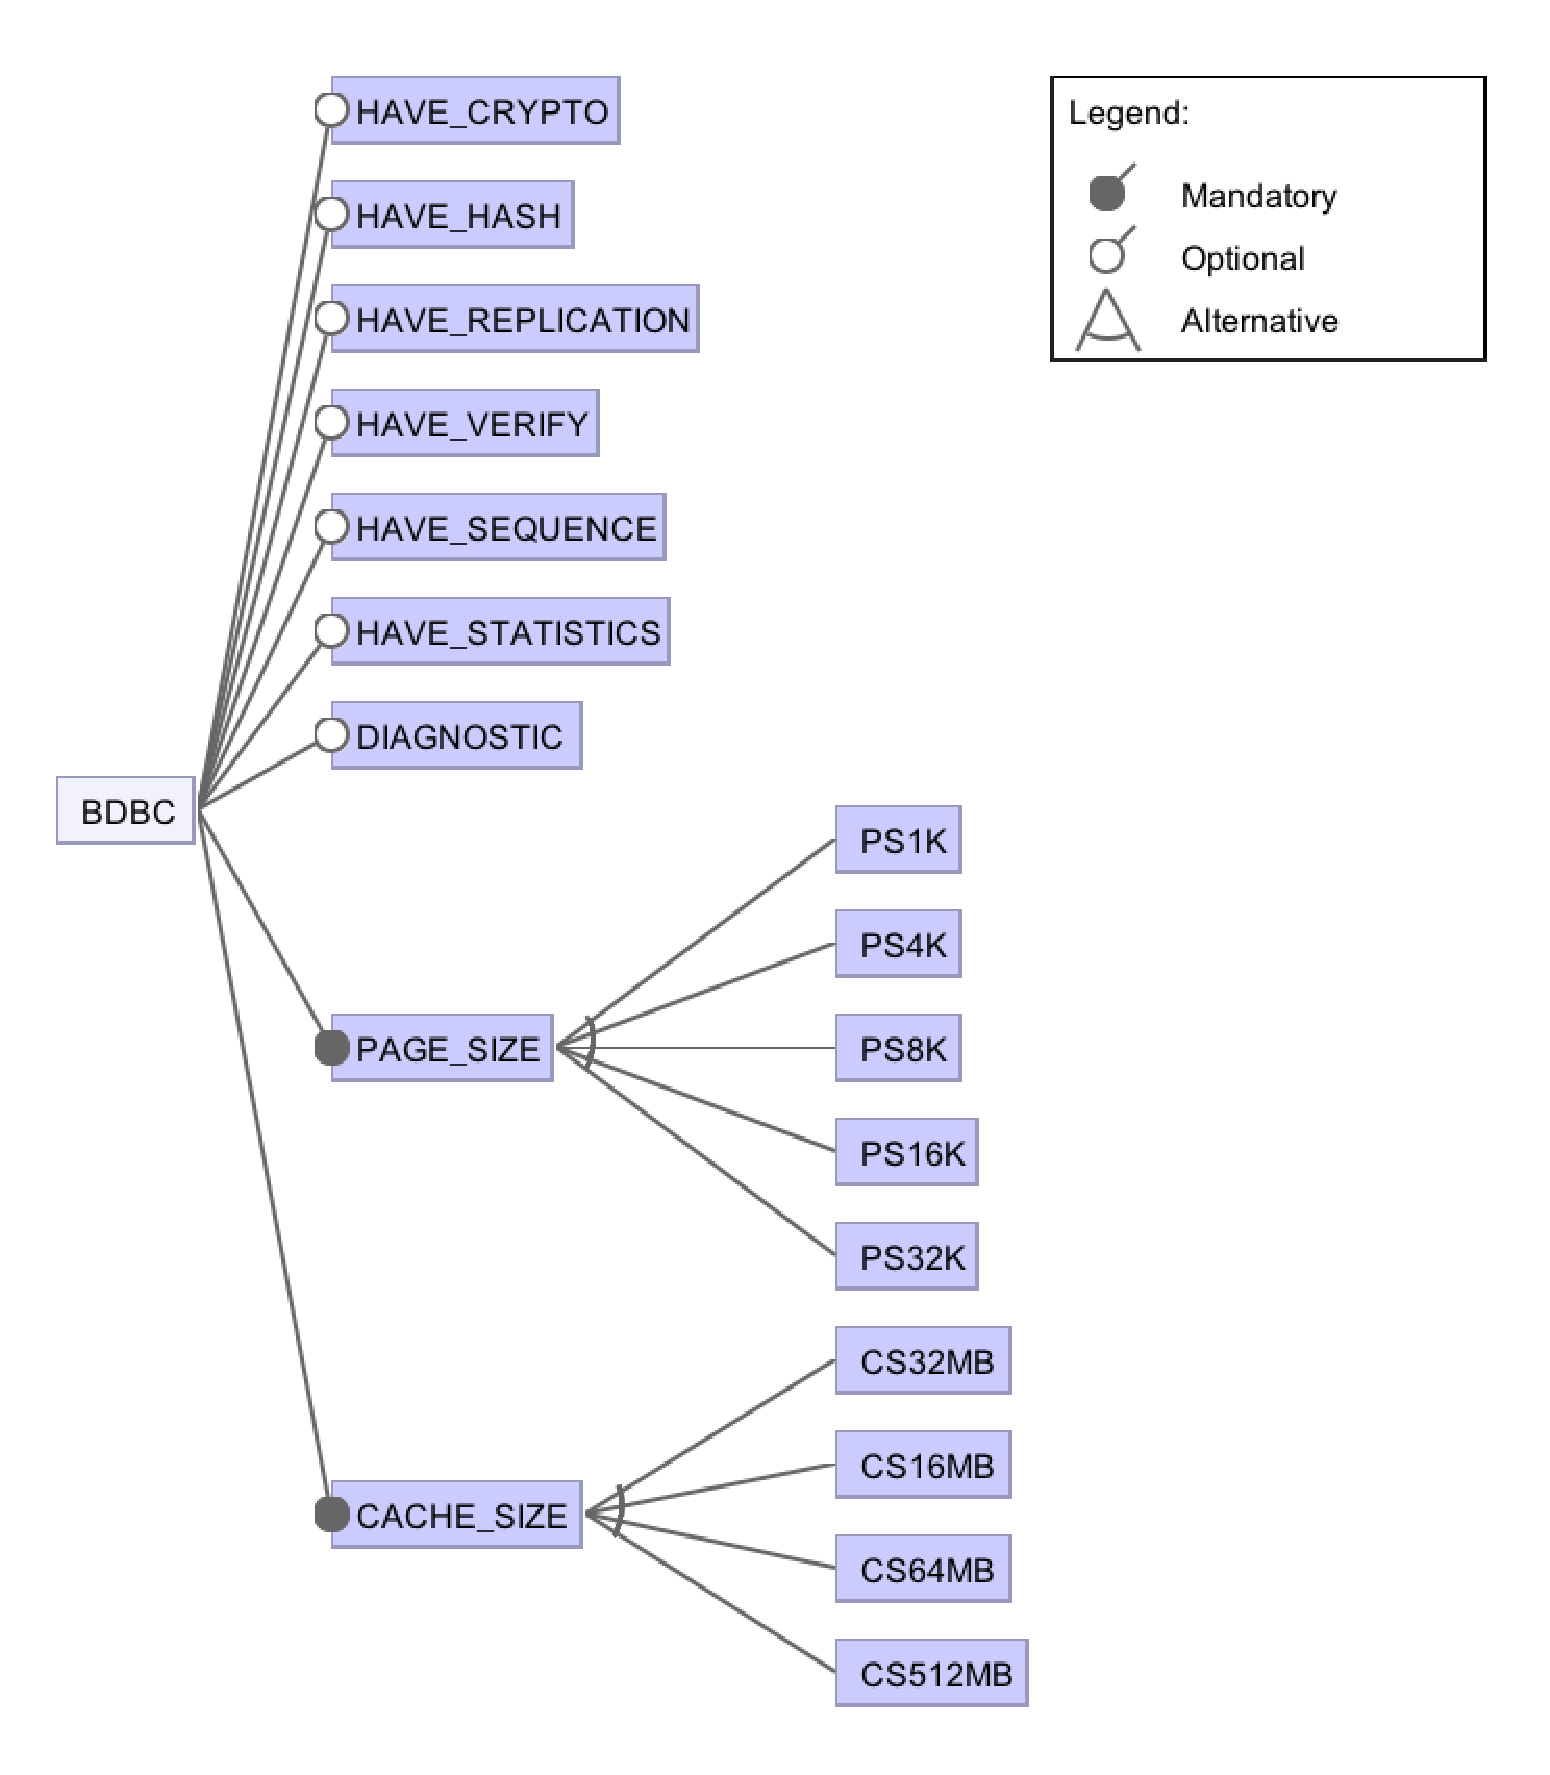
\includegraphics[width=1\linewidth]{Figures/BDBC.eps}
\caption{ Berkeley database feature model   (``C'' version). }\label{fig:bdbc}
\end{figure}
    


\begin{figure}[!t]
\scriptsize
\begin{tabular}{llllll}
  \hline
Project & Domain & Lang. & LOC & Features & Config\\\hline
Berkeley DB(BDBC)   & Database & C & 219,811 & 18 & 2560\\
Berkeley DB(BDBJ)   & Database & Java & 42,596 & 32  & 400\\
Apache & Web Server & C & 230,277 & 9 & 192\\
SQLite & Database & C & 312,625 & 39 & 3,932,160\\
LLVM & Compiler & C++ & 47,549 & 11 & 1024\\
x264 & Video Enc. & C& 45,743 & 16 & 1152\\\hline
\end{tabular}
\caption{Feature models studied in this paper. For details on these systems,
see \fig{systems}.}
\label{fig:subjectsystems}
\end{figure}


\begin{figure}\small
\begin{tabular}{|p{.95\linewidth}|}\hline
\textbf{Berkeley DB CE} is an embedded database system written in C. It is one of the most deployed databases in the world due to its low binary footprint and its configuration abilities. We used the benchmark provided by the vendor to measure response time.

\textbf{Berkeley DB JE} is a complete re-development in Java with full SQL support. Similarly, we used a benchmark provided by the vendor measuring response time.

\textbf{Apache} is a prominent open-source Web server that comes with various configuration options. To measure performance, we used the tools autobench and httperf to generate load on the Web server. We increased the load until the server could not handle any further requests and marked the maximum load as the performance value.

\textbf{SQLite} is an embedded database system deployed over several millions of devices. It supports a vast number of configuration options in terms of compiler flags. As benchmark, we used the benchmark provided by the vendor and measured the response time.

\textbf{LLVM} is a compiler infrastructure written in C++. It provides configuration options to tailor the compilation process. As benchmark, we measured the time to compile LLVM's test suite.

\textbf{x264} is a video encoder in C that provides configuration options to adjust output quality of encoded video files. As a benchmark, we encoded the Sintel trailer (735\,\%MB) from avi to the xH.264 codec and measured encoding time.\\\hline
\end{tabular}
\caption{Systems studied in this paper.}\label{fig:systems}
\end{figure}



\section{Background}  

\subsection{Product Lines as Feature Models}
We represent the software systems using Kang's feature model (FM) notation. 
A feature model defines all valid feature combinations of a customizable system. 

As shown in the Figure~\ref{fig:bdbc} a feature model can be presented as a tree like structure that defines relationships among features.   Features are represented as a set of binary decision variables. 

A feature, when selected, corresponds to 1, and 0 otherwise. All the features of a system is represented a {\em configuration} vector  $C_i= <f_1, f_2, ...,f_N>$, 
where N is the number of features of the product line.  
    
Feature models can be far more elaborate than \fig{bdbc}. 
A feature model of the LINUX kernel~\cite{sayyad13b} contains thousands of features and hundreds of thousands of  {\em cross-tree constraints}; i.e. choices in one branch that rule out choices in other branches. 
Without those constraints, it takes linear time to generate possible products via a simple
top-down descent of the model. With those constraints, product generation becomes NP-hard and can
 defeat state-of-the-art theorem provers~\cite{pohl11} (particularly for larger feature models).
 
 
 
In practice, not all feature models are as complex as in one of LINUX.
\fig{subjectsystems} details the feature models used in this study. While
they seem to be small (just a few dozen features), the last column in that table lists hundreds
to millions of configurations they can generate.


\subsection{Predicting Run-times}\label{sect:addit}
How can we predict the run-times of products generated from such high-level descriptions
as \fig{bdbc}? The literature offers two approaches: a {\em maximal sampling} and a {\em minimal sampling} method.

In the {\em maximal sampling} method, we compile all  possible configuration and record the associated run-times. Maximal sampling  can be impractically slow.
For example, the run-time data used in this paper required  26 days of CPU time to collect (and much longer, if we also count the time required
 for compiling the code prior to execution). 
 Other researchers have commented that,  in 
 real world scenarios, the cost of acquiring optimal configuration is overly expensive and time consuming \cite{weiss2008maximizing}.
 
 When collecting run-times on all configurations is impractical,  {\em minimal sampling } 
 is required to intelligently select and execute   just enough configurations samples to build
 predictive models.
 Zhang et al.~\cite{zhang2015performance} approximate the
 systems as a Fourier series, after which they can derive an expression showing how many configurations must be studied
 to build predictive models with error $\epsilon$. While a theoretically satisfying result, that approach still needs thousands to hundreds of thousands of executions of sample
 configurations.  

Another set of approaches are the four "additive" {\em minimal sampling} methods for Siegmund et al.~\cite{siegmund2012predicting}.
Their first method, called feature-wise (FW) is their basic method and 
Three of these methods are    elaborations of their basic method, called feature-wise (FW)
selection.

To explain FW, we note that from a product line, it is theoretically possible to enumerate all (or many) of the legal configurations\footnote{Though in practice, this can be very difficult. For ex. in models like Linux Kernel such an enumeration is practically impossible ~\cite{sayyad13b}}. 
Each such
configuration is a vector of $n$ booleans where $n_i$ indicates if this configuration uses feature $n_i$ (and
an example of ``feature'', see the leaf nodes of \fig{bdbc}).
Using this information it  is possible to isolate examples of how much each feature individually contributes to the total runtime:
\be
\item Find a pair of  configurations $C_1,C_2$  where $C_2$ uses exactly the same features as $C_1$, plus just one  extra feature $f$.
\item Set the runtime $\Pi(f)$ for feature $f$ to be the difference in the run-times between $C_2$ and $C_1$.
\item The runtime  for a new configuration  $C_i=\{f_1,f_2,f_3,,,\}$, that has not been sampled before,  is the sum of the runtime of its features; i.e.
\begin{equation}
  \Pi(C_i) = \sum_{f_j \in C_i}\Pi(f_j)  
\end{equation}
\ee

Further to the first point, when many pairs $C_1,C_2$ satisfy the criteria of point~1, Siegmund et al. used the 
pair that mentions the {\em smallest} number of features. Their basic {\em FW} minimal sampling method 
just compiles and executes just these smallest $C_1,C_2$ configurations. 

Siegmund et al. also offered three extensions to the basic method. All these extensions are based on sampling
not just the smallest $C_1,C_2$  pairs but also any configurations with {\em interactions}. 
All the following minimal sampling policies compile and   execute legal configurations selected via one of three heuristics:
\bi
\item[{\em PW (pair-wise):}] Given the space of all configurations, if two configurations contain the same pairs of setting to features, 
ignore one of the them. 
\item[{\em HO (higher-order):}] Select extra configurations that 
mention three features $a,b,c$ where   $(a,b)$ and $(b,c)$ and $(a,c)$ are known pair-wise features.
\item[{\em HS (hot-spot features):}] Select extra configurations that contains features that are used very
frequently along with features that are rarely used. 
\ei

The advantage of these additive methods are that, unlike  Zhang et al. these additive methods require only dozens to hundreds of samples. That said, as shown by the experiments later in this
paper, they produce estimates with large mean error and larger variance than the \what method proposed by
this paper.
 

\subsection{Spectral Learning}\label{sect:spect}

The minimal sampling method explored in this paper is based on a spectral learning algorithm
that  explore the spectrum (eigenvalues) of a distance matrix between  configurations.
In theory, such spectral learners are a better way to handle noisy, redundant and tightly inter-connected variables, for the following reasons.
When data sets have many irrelevancies   or closely associated data parameters $d$, then
only a few $e \ll d$ eigenvectors are required to characterize that data.
In that reduced space:
\bi
\item
Multiple inter-connected variables $i,j,k \subseteq d$ can be represented
by a single eigenvector.
\item
Noisy variables from $d$ are
ignored since they  do not contribute to the signal in the data.
\item
Variables  become (approximately) parallel lines
in $e$ space. For  redundancies \mbox{$i,j \in d$}, we
can ignore $j$
since effects that change over $j$ also
change in the same way over $i$.
\ei
That is, in theory, samples of configurations drawn via an eigenspace sampling method
would not be confused by noisy, redundant or tightly inter-connected variables. Accordingly,
we expect predictions built from that sample to have  lower mean errors and lower variances on that error.

Spectral methods have been used before for a variety of data mining applications~\cite{kamvar2003spectral}.
Algorithms like PDDP~\cite{boley98} use spectral methods such as principle component analysis (PCA) to
recursively divide data into smaller regions.  Software analytics researchers such as Theisen et al.~\cite{Theisen15}  use spectral methods (again, PCA) as a pre-processor prior to data mining  to reduce noise in software-related data sets.
However, to the best of our knowledge, spectral methods have not been used before in software engineering as a basis 
of a minimal sampling policy.



\what is somewhat different from other spectral
learners explored in, say, image processing applications~\cite{shi00}.
The image processing papers do not address
our key contribution presented in this paper  (defining
 a minimal sampling policy to predict run-times).
Also,
standard spectral method requires some $O(N^2)$ matrix multiplication to compute, say, the components
of PCA~\cite{ilin10}. Worse, in the case of hierarchical division methods such as PDDP,
that polynomial time inference must be repeated at every level of the hierarchy.
Competitive results can be achieved
using an $O(2N)$ analysis that we have developed previously~\cite{me12d}, which is  based on  a heuristic proposed by
Faloutsos and Lin~\cite{Faloutsos1995}
(which
Platt has
  shown computes a Nystr\"om
  approximation to the first component of
  PCA~\cite{platt05}).
  
  This approach inputs
$n$
examples $n_1,n_2,..$. The FASTMAP heuristic
picks any
point $n_i$ at random and  finds
 the point  {\em West}~$\in n$ that is
furthest away

from $n_i$.
FASTMAP then
finds the point {\em East}~$\in n$
that is furthest from {\em West}.
We say that the line between {\em West} and {\em East} has  length  
$c=\mathit{dist}(\mathit{West},\mathit{East})$.
Using this  approach, \what uses FASTMAP recursively to divide all the configurations as follows.
We iterate over $n_i \in n$
to find
$a=\mathit{dist}(n_i,\mathit{West})$,
$b=\mathit{dist}(n_i,\mathit{East})$,
$x=(a^2 + c^2 - b^2)/(2c)$.
This  $x$ value is the projection of $n_i$
on the line  running  from {\em East} to {\em West}.  We divide
the examples based on the median value of the projection($x$),
then recurse on each half. The recursion on
$n$ initial
examples stops when a sub-region
contains less that  $M$ examples (e.g. 
$M=\sqrt{|n|}$).
We explore this approach for three reasons
\bi
\item
{\em It is very fast}:
This process requires only $2*|n|$ distance comparisons
per level of recursion, which is far less than the $O(|n|^2)$
required by PCA~\cite{Du2008}
or other  algorithms such as K-Means~\cite{hamerly2010making}.
\item
{\em It is not domain specific}:
This approach is general unlike traditional PCA. We do not make any assumption that all variables are numeric. As shown in equation 2, we can approximate distances for both numeric and non-numeric data.

\begin{equation}
    dist(x, y) = 
    \begin{cases}
        \sqrt{\sum_i(x_i-y_i)^2},& \text{if $x_i$ and $y_i$ is numeric}\\
        \begin{cases}
            0, & \text{ if $x_i$ == $y_i$}\\
            1, & \text{ otherwise}\\
        \end{cases}
        ,& \text{if $x_i$ and $y_i$ is boolean}\\
    \end{cases}
\end{equation}

\item
{\em Explore the underlying dimension of the search space (configuration space)}:
This technique explores the underlying dimension (first principal component) without getting confused by noisy, related and highly associated variables (see section 3.3).

\ei

\subsection{Spectral Sampling}\label{sect:sample}
When the above clustering method terminates, our  sampling policy (which we will call $S_1$:Random) is then applied:
\begin{quote}
$S_1$: Random sampling: Compile and execute one  configurations,  picked at random, from each leaf cluster.
\end{quote}
We use this sampling policy since, later in this paper, we show $S_1$:Random sampling performs better than:
\bi
\item $S_2$: East-West sampling: compile and execute the {\em East} and {\em West} poles of the leaf clusters;
\item $S_3$: Exemplar sampling: compile and execute all items in all leaves and return the one
with lowest run-time score.
\ei
Note that $S_3$ is {\em not} a {\em minimal} sampling policy (since it executes all configurations). 
We use it here as one  baseline
against which we can compare the other, more minimal, sampling policies (note that, in the results
that follow, we also compare our 
sampling methods against another baseline--
using information gathered after executing
all configurations).

\subsection{Regression Tree Learning}
After collecting the data using one of the sampling policies, we then use the CART regression tree learner \cite{breiman1984} to build a predictor for run-times. Regression tree learners seek the attribute range split that most increases
our ability to make accurate predictions.
CART explores splits that divide $n$ samples  into   with $n_1$ and $n_2$ samples, where each sample  has a  standard deviation on the target variable of $\sigma_1$ and  $\sigma_2$.
CART finds the ``best'' split; i.e. the one that minimizes $\frac{n_1}{n}\sigma_1 + \frac{n_2}{n}\sigma_2$.
Using this best split, CART divides the data, then recurses into each split.
 

The validity of the predictors built by CART  is then tested on testing data. There is no intersection between the training data (spectral learning processing) and the testing data (see below for details). For each  test item, we find out how long it {\em actually} takes to run and compare that
to the {\em prediction} from CART. The resulting prediction error is then computed using:
\begin{equation}\label{eq:err}
\mathit{error}=\frac{\mathit{abs}(\mathit{predicted} - \mathit{actual})}{\mathit{actual}}*100
\end{equation}

\section{Research Questions} 
In summary, \what  combines:
(1) the FASTMAP method of Faloutsos and Lin~\cite{Faloutsos1995};
(2)~a spectral learning algorithm initially   inspired by    Boley's PDDP system~\cite{boley98}, which we modify
by replacing  PCA with FASTMAP (prior work have called this
method ``WHERE''~\cite{me12d});
(3)~the $S_1$:Random sample method that explores the leaf clusters found by this recursive division;
and (4)~the CART regression tree learner that converts the data from the samples collected by $S_1$:Random
into a runtime prediction model~\cite{breiman1984}.
That is,
\begin{center}
\begin{tabular}{rcl}
WHERE& = &PDDP - PCA + FASTMAP\\ 
\what& =  & WHERE + $S_1$:Random + CART
\end{tabular}
\end{center}
This combination of methods has not been previously explored in the
software engineering literature but is promising because it explores the underlying dimension of the space without getting confused by noisy, redundant and highly associated variables (see section 3.3).


Since our model explores the spectral space, it might be true that only small
number of samples are required to explore it all.
But, a model built from a very small sample of the available data might
be very inaccurate and unstable; i.e. it may exhibit very large mean errors and standard deviations on the error.

Also, if we learn models from very small regions of the training data,
then it is  possible that that learner will miss {\em trends} in the data
between the sample points. Such trends are useful when building {\em optimizers};
i.e. devices that input one configuration and propose an alternate
configuration that has (say) faster run-times. Such optimizers might
need to evaluate hundreds to millions of alternate configurations. 
To speed up that process, optimizers can use a {\em surrogate model}\footnote{Also known as response surface methods, meta models, or emulators.}
that  mimics the outputs of a system of interest, while being computationally cheap(er) to evaluate~\cite{loshchilov13}. For example, when optimizing
run-times, we might ask the CART  for a performance
prediction (rather than compile and execute
configurations).  Note that such surrogate-based
reasoning critically depends on how well the surrogate can guide optimization.


Therefore, to assess our sampling policies, we must compare:
\bi
\item Performance scores (run-times) generated from our minimal sampling policy;
\item The variance of the performance scores (to check for the stability
of those performance predictions);
\item The optimization support offered by the performance predictor i.e. can the model work in tandem with other off-the-shelf optimizers to generate useful solutions
\ei
The above concerns leads to four research questions:
\bi
\item {\bf RQ1:} {\em Can  \what  +$S_1$:Random spectral learning generate good predictions after only
executing a small number of configurations?}
\ei
Here, by ``good'' we mean that the predictions found via sampling with \what+$S_1$:Random are as good, or better,
as those generated from far more samples.
\bi
\item {\bf RQ2:} {\em
Does less data used in building the models lead to large variability in the predicted values?}
\item {\bf RQ3:} {\em
Can ``good'' surrogate models (to be used in optimizers)
be built from minimal samples?}
\ei
Note that {\bf RQ2, RQ3} are of particular concern with our approach
since we are sampling so little from the total space of possible
configurations.
\bi
\item {\bf RQ4:} {\em Compared to the state-of-the-art in minimal sampling for
learning run-time predictors from product lines, how good is \what with $S_1$:Random?}
\ei
To answer this last question, we will compare \what with $S_1$:Random
          against the FW, PW, HO, HS heuristics of Siegmund et al. (described above in \tion{addit}).
 
\section{Experiments}

\subsection{Reproduction Package}

All the materials required to reproduce this work are available at \url{https://goo.gl/689Dve}.

\subsection{Case Study Materials}

This study explores feature models, along with the run-time measurements obtained from real time measurements, of the products lines listed in \fig{subjectsystems}.
Also, to compare our results from minimal sub-sampling to those obtained 
from a larger sample, we use data sets showing the run-times associated with
compiling and executing {\em nearly all} configurations\footnote{http://openscience.us/repo/performance-predict/cpm.html}.

We say {\em nearly all} configurations, for the following reasoning. For 
$\frac{5}{6}$ths of our case studies, the number of possible configurations
was not large (192 to 2560). However, the SQLite product line has 3,932,160 
possible configurations-- which is an impractically large number of configurations to explore. Hence, for SQLite, we use the 4500 samples that could
be collected in one day of CPU time (and, in the results shown below,
we will pay particular attention to the variance of the SQLite results).

\subsection{Experimental Rig}


{\bf RQ1,RQ2} require the construction and assessment of numerous runtime predictors from small samples
of the data. The following rig implements that construction process.

For each product line, we built a table of data, one row per valid configuration. We then run all configurations of all software systems
and record the performance scores (i.e., that are invoked by a benchmark).
The exception is SQLite in which we measure only the
configurations needed to detect interactions and additionally
100 random configurations to evaluate the accuracy of
predictions.  
To this table we added a column showing the performance score (obtained from the real time measurements) for each configuration (refer to section 2.

Next, 20 times, we repeated the following procedure (the figure of 20 repeats was
selected using the central limit theorem). Note that the following rig ensures that
we never test any prediction model on the data used to build that model.
\bi
\item For each  product line in \{BDBC, BDBJ, Apache, SQLite, LLVM, x264\},
\bi
\item Randomize the order of the rows in their table of data;
\item For $X$ in \{10, 20, 30... , 90\};
\bi
\item Let {\em Train} be the first $X$\% of the data 
\item Let {\em Test} be the rest of the data;
\item Pass {\em Train} to \what to find a sample of configurations;
\item Determine the run-times associated with those configurations (in our rig, that is a table lookup and when
this approach is used in practice, this would entail compiling and executing the software product).
\item Using the {\em Train}  data (and their run-times), build a defect predictor using CART.
\item Using {\em Test}, assess the predictor using the error 
measure of \eq{err}.
\ei
\ei
\ei
{\bf RQ2} required testing the standard deviation of the predictions. To support that test, we:
\bi
\item Determine the $X$-th point in the above experiments where all predictions stop improving;
\item Measure the standard deviation of the error at that point, across our 20 repeats.
\ei
As shown in figure \ref{fig:sampling_accuracy}, all our results plateaued after studying $X=40$\% of the valid configurations
 \footnote{Just to clarify one frequently asked question about this work, we note
that our rig ``studies'' 40\% of the data, we do not mean that our predictive models
 require access to run-times from the 40\% of the data. Rather, by ``study'' we mean   reflect 
 on a sample of configurations to determine what minimal subset of that
sample deserves to be compiled and executed.}.
 Hence to answer {\bf RQ2}, we will compare all 20 predictions at $X=40$\%.
 
{\bf RQ3} requires using the regression tree learned in this way as a {\em surrogate model} within an optimization process. To study this research question, we:
\bi
\item Take   $X=40\%$ of the configurations;
\item Apply \what with $S_1$:Random to build a CART model using some minimal sample taken from that 40\%;
\item Used that CART model within some standard optimizers while searching for 
configurations with least runtime;
\item  Compare the faster configurations found in this manner with the fastest configuration
known for that product line.
\ei
This last item requires access to some ``ground truth'' of run-times for a very
large number of configurations. For this experiment, we have access to that ground truth
(since we have access to nearly all the configurations). While that ground truth is required for this
validation study, we note that, once our methods satisfy this validation study,
they would not not be needed in if practitioners choose to use \what in their own work.

As to the optimizers used in this second experiment, for the sake of completeness, we explored
a range of optimizers (see Appendix).  Normally,
it would be  reasonable to ask
why we used those three, and not the hundreds of other 
optimizers described in the literature~\cite{fletcher13,harman12}. However,
as shown below, all these optimizers in this
domain exhibited  very similar
behavior (all found configurations were very nearly
best case performance). Hence, the specific
choice of optimizer is not a critical
variable in  our analysis.


\section{Results}


\begin{figure}[!t]
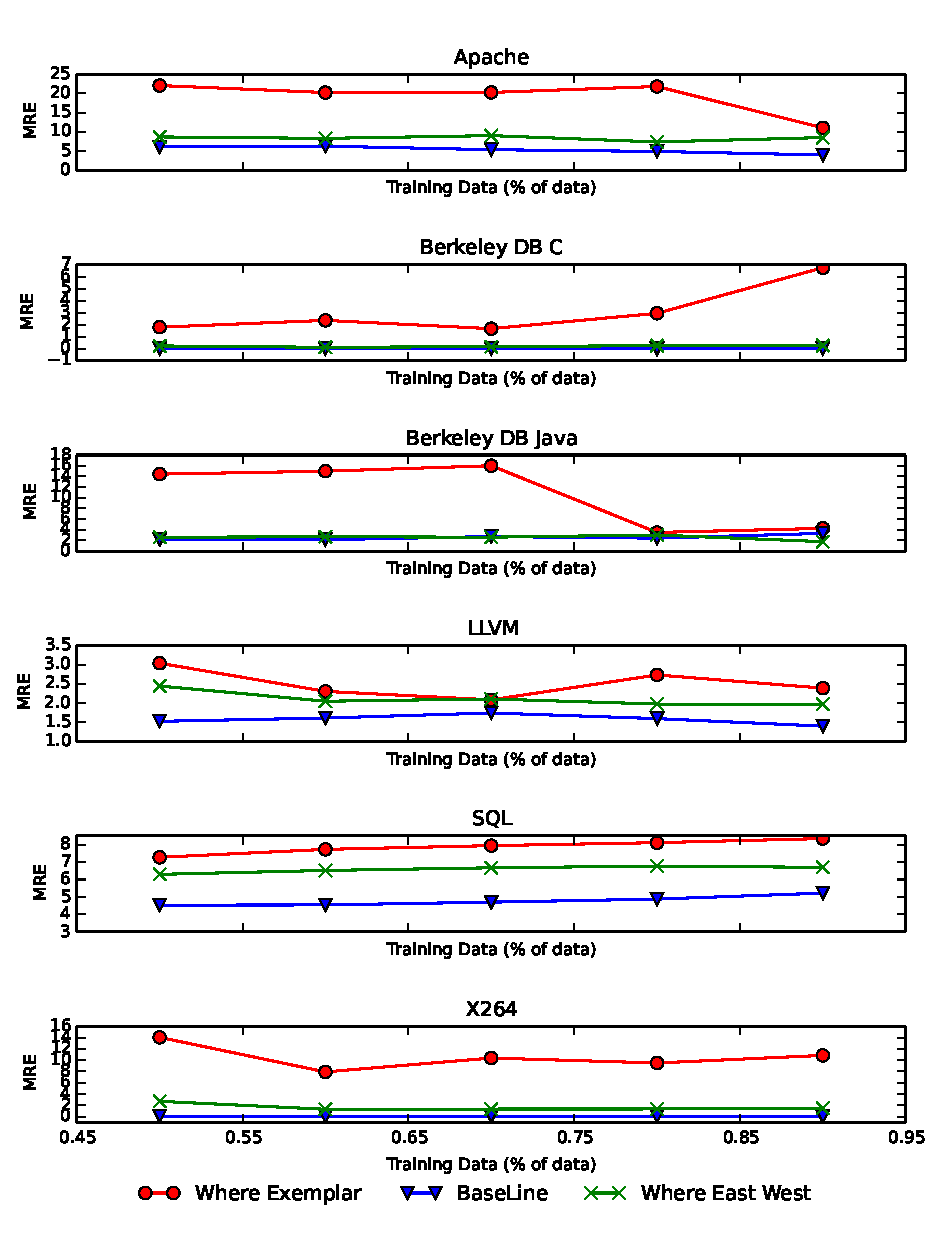
\includegraphics[width=0.9\linewidth]{Figures/SamplingAccuracy.eps}
\caption{Error seen in the predictions made by \what with four different
sampling policies. Note that. on the y-axis,  {\em lower} errors are {\em better}.}
\label{fig:sampling_accuracy}
\end{figure}

\subsection{RQ1}
{\em Can  \what  +$S_1$:Random spectral learning generate good predictions after only
executing a small number of configurations?}

\fig{sampling_accuracy} shows the mean errors of the predictors learned
after taking $X$\% of the configurations, then asking  \what and some sampling method
to (a)~find what configurations to execute; then (b)~asking CART to build a predictor
using that execution information. The horizontal axis of those plots shows what $X$\%
of the configurations are studied and the vertical axis shows the mean relative error (from \eq{err}).
In that figure:
\bi
\item
The \textcolor{blue}{{\bf blue}} lines on \fig{sampling_accuracy} show a {\em baseline} result
where data from the run-times of 100\% of  configurations from 0 to $X$ were used by CART
to build a runtime predictor.
\item
The other lines show the results using the sampling methods defined in \tion{sample}.
Note that these sampling methods only used  runtime data from
some subset of 100\% of the run-times seen in configurations
from 0 to X\%.
\ei


Note that, in  \fig{sampling_accuracy}, {\em lower} y-axis values are {\em better} since this shows lower
prediction errors. We found that:
\begin{itemize}

\item Some product lines exhibit large variances in their fault rate, below $X=40$\% (see the BDBC and BDBJ
results).
\item Above $X=40$\%, there is little effect on other overall change of the sampling methods.
\item
Nearly always, the {\em exempler} sampling method $S_3$ shows  highest overall error 
so it cannot be recommended.
\item Always, the  {\bf blue baseline} results  had lowest errors- which is to be
expected since predictors built on the baseline have access to all data.
\item
Usually, the error of  $S_1$:Random and $S_2$:EastWest, are within $5$\% of the {\em baseline} results.
Hence, we can recommend these two minimal sampling methods.
\end{itemize}
\fig{Evaluations} comments on one which  of    $S_1$:Random or $S_2$:EastWest we should recommend.
This figure displays data taken from the $X=40$\% point of \fig{sampling_accuracy} and displays
how many run-times of configurations are needed by our sub-sampling methods (while
reflecting on the configurations seen in the range $0\le X \le 40$. Note that:
\bi
\item
The {\em Exemplar} sampling policy needs up to thousands of run-time points, 
so it cannot be recommended as
minimal sampling
policy;
\item The {\em East-West} sampling policy needs twice as much run-time information as 
the $S_1$:Random {\em random} policy (since $S_2$ uses {\em two} samples per leaf cluster  while
$S_1$:Random only uses {\em one}).
\item $S_1$:Random only needs run-time information on a few dozen (or less) configuration to generate
the predictions with the lower errors seen in \fig{sampling_accuracy}.
\ei

\begin{myshadowbox}
Combining \fig{sampling_accuracy} and \fig{Evaluations} results, we conclude that:
\bi
\item
$S_1$:Random is our preferred spectral sampling method;
\item
The answer to {\bf RQ1} is ``yes'' since using \what +\\$S_1$:Random we can (a)~generate runtime predictors
using just a few dozens examples of run-times; and (b)~those predictions have errors
within 5\% of the error seen if predictors built from information about all run-times.
\ei
\end{myshadowbox}

\begin{figure}[!t]
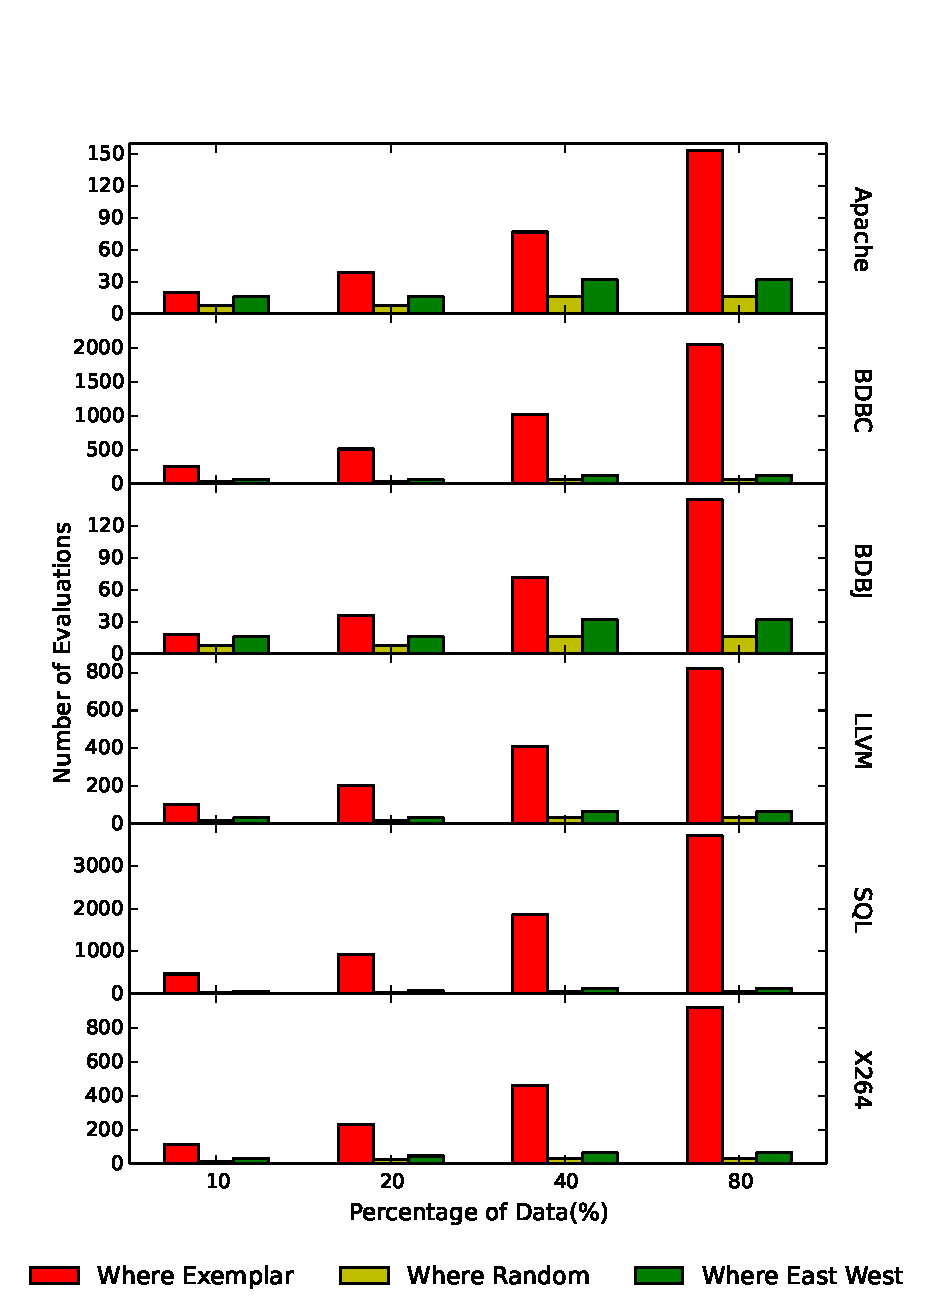
\includegraphics[width=0.9\linewidth]{Figures/evaluation_graph.eps}
\caption{ Comparing evaluations of different sampling policies. We see that the number of configurations evaluated for $S_2$:EastWest is twice as much as $S_1$:Random, since it selects 2 points from each cluster where as  $S_1$:Random only selects one }\label{fig:Evaluations}
\end{figure}


\subsection{RQ2}

{\em
Does less data used in building the models lead to large variability in the predicted values?}\\

Two competing effects can lead to increased, or less,  variability  in 
runtime predictions:
\bi
\item
The less we sample configuration space,
the less we constrain model generation in that space. Hence, models learned
from too few samples can exhibit large variance (see the examples of that effect,
in the introduction). 
\item
A compensating effect can be introduced by sampling from spectral space
since that space contains fewer confusing variables than that raw data.
\ei
\fig{Variance} reports which one of these two competing effects are dominate. 
The \fig{sampling_accuracy} shows that after some initial fluctuations,
after seeing $X=40$\% of the data, the variability in predictions falls away to nearly zero.


\begin{figure}[!t]
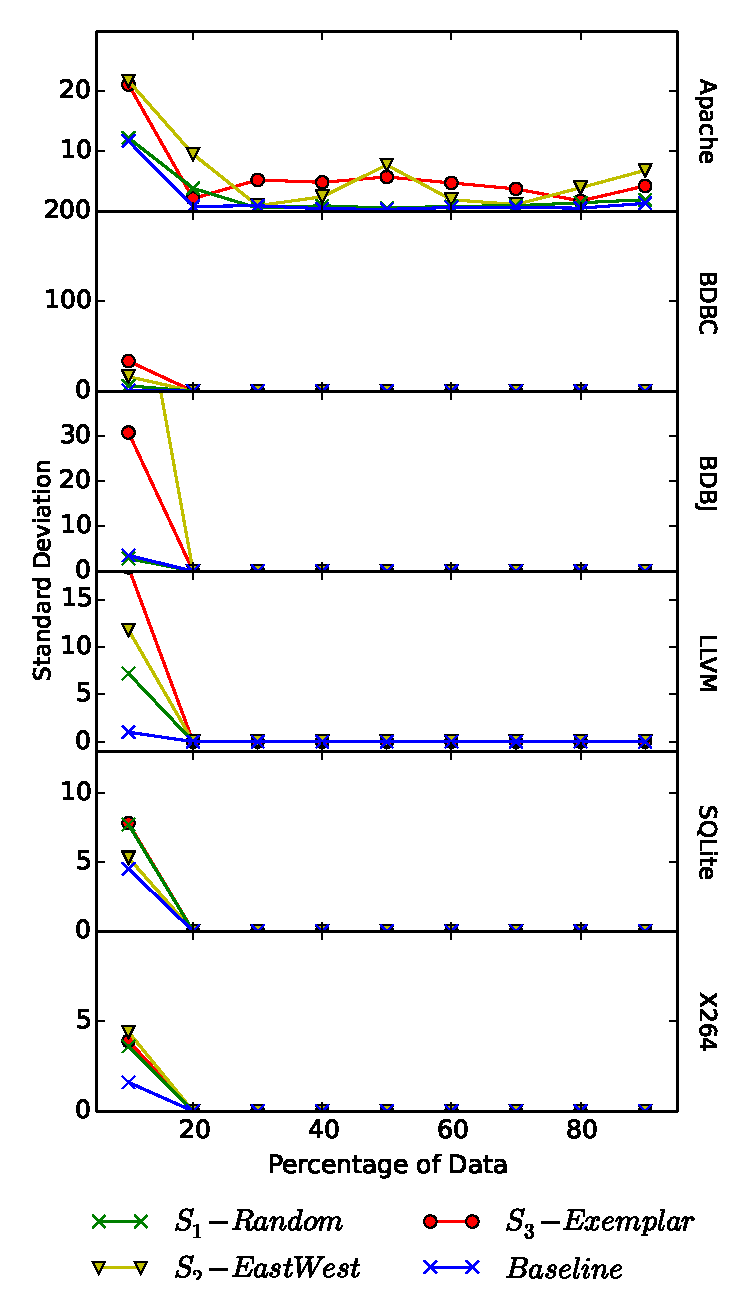
\includegraphics[width=0.9\linewidth]{Figures/Variance.eps}
\caption{Standard deviations seen at various points of  \fig{sampling_accuracy}.}\label{fig:Variance}
\end{figure}

\begin{myshadowbox}
Hence, we answer {\bf RQ2} as ``no'', selecting a small number of samples does not increase variance (at least to say, not in this domain).
\end{myshadowbox}


\subsection{RQ3}

 {\em
Can ``good'' surrogate models (to be used in optimizers)
be built from minimal samples?}

The answers to {\bf RQ1,RQ2} recommend the use of \what+$S_1$:Random to build runtime predictors from a very small sample
of the data. {\bf RQ3}
asks if that predictor can be used by an optimizer to infer what {\em other} configurations might generate very fast run-times?
To answer this question,  we ran  a random set of 100 
configurations, 20 times, then based that baseline to three optimizers (GALE and two 
other optimisers,  details in Appendix.


When these three optimizers mutated existing configurations to suggest new ones,
those mutations were checked against the feature model. Any mutants that violated the feature model constraints were rejected
and the survivors were ``evaluated'' by asking a surrogate
(the  CART regression tree learned from \what+$S_1$:Random, built using the methods of {\bf RQ1}).
These evaluations either rejected the mutant or used it in generation $i+1$, as the basis for a search for more, possibly
better  mutants.

\fig{performance_graph} shows the configurations found by GALE projected onto the ``ground truth'' of the run-times of nearly
all configurations. Again note that, while we use that ``ground truth'' for the validation of these results, our optimizers only
used a very small percent of that ground truth in their search for fastest configurations (see the \what + $S_1$:Random
results of \fig{Evaluations}).


\begin{figure}[!t]
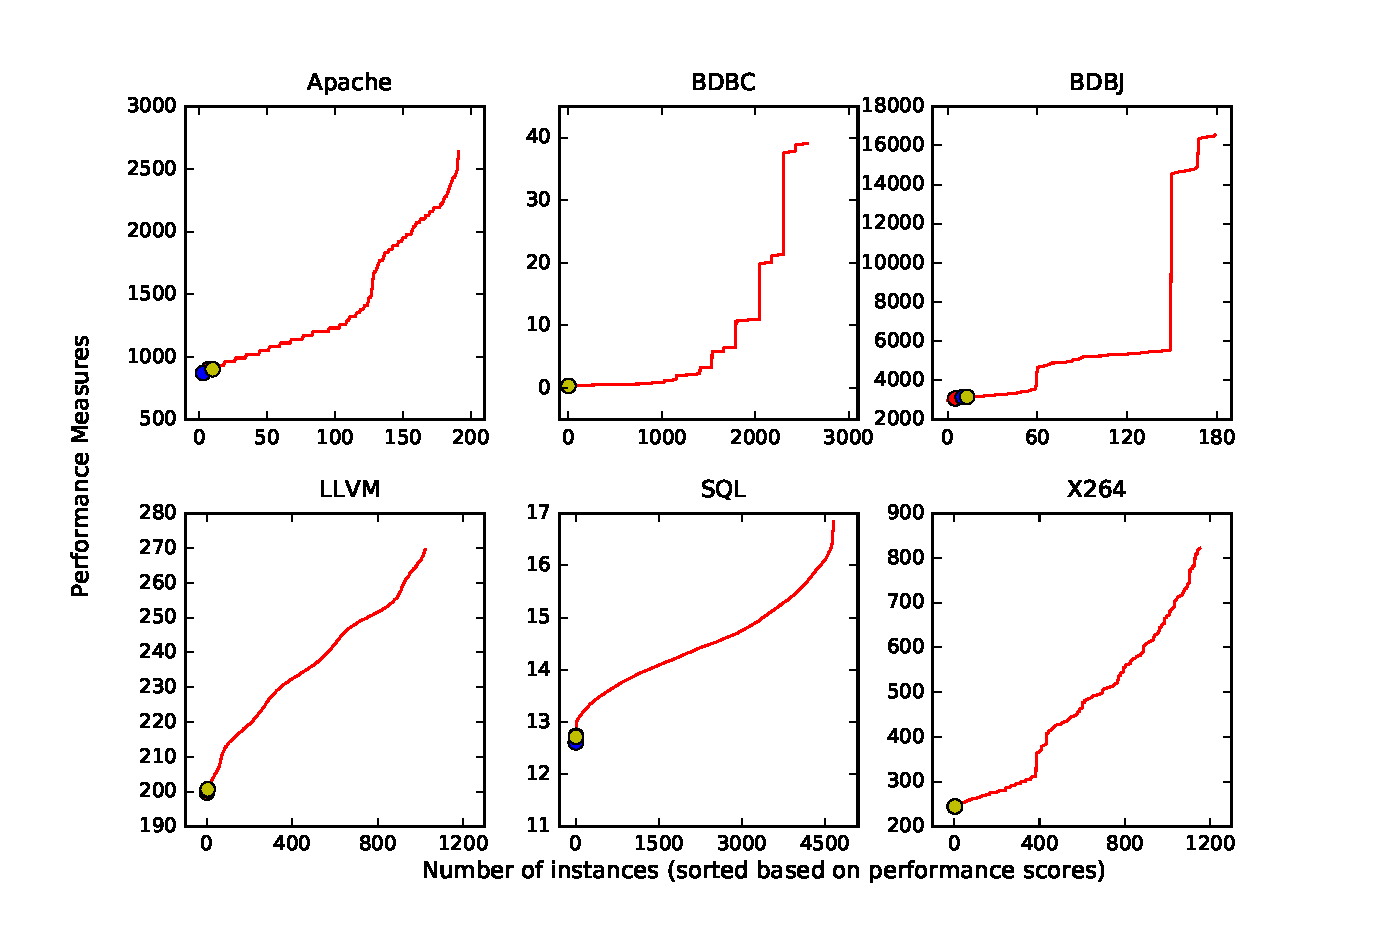
\includegraphics[width=0.9\linewidth]{Figures/optimizer_result.eps}
\caption{Solutions found by GALE (shown as points) laid against the ground truth (all known configuration run-times) with the exception of SQLite, as this dataset does not contain the exhaustive set of configurations and the corresponding performance scores.}\label{fig:performance_graph}
\end{figure}


The important feature of \fig{performance_graph} is that all the optimized configurations fall within 1\% of the fastest
configuration in the ground truth (see all the left-hand-side dots on each plot).. \fig{external_validity} compares GALE's performance to that of the two other optimizers
used in this study. Note that the performances are nearly identical which leads to two conclusions:
\be
\item The answer to {\bf RQ3} is ``yes''-- for optimizing run-times, we can use surrogates built from very few runtime samples;
\item That first point is not critically effected by the choice of optimizer.  
\ee


\begin{figure}
\resizebox{3.3 in}{!}{

\begin{tabular}{|l@{~}|l@{~}|l@{~}|l@{~}|l@{~}|l@{~}|l@{~}|l@{~}|l@{~}|l@{~}|l@{~}|l@{~}|l|}
\hline
\multirow{2}{*}{Searcher} & \multicolumn{2}{l|}{Apache} & \multicolumn{2}{l|}{\begin{tabular}[c]{@{}l@{}}Berkeley \\ DB C\end{tabular}} & \multicolumn{2}{l|}{\begin{tabular}[c]{@{}l@{}}Berkeley \\ DB Java\end{tabular}} & \multicolumn{2}{l|}{LLVM} & \multicolumn{2}{l|}{SQLite} & \multicolumn{2}{l|}{X264} \\ \cline{2-13} 
                          & $\mu$         & IQR        & $\mu$                                 & IQR                                  & $\mu$                                   & IQR                                   & $\mu$       & IQR        & $\mu$      & IQR        & $\mu$       & IQR        \\ \hline
GALE                      & 870            & 0          & 0.363                                 & 0.004                                & 3139                                     & 70                                    & 202       & 3.98       & 13.1     & 0.2411     & 248      & 3.3       \\ \hline
DE                        & 840            & 0          & 0.359                                 & 0.002                                & 3139                                     & 70                                    & 200       & 0          & 13.1      & 0          & 244       & 0.003      \\ \hline
NSGA2                     & 840            & 0          & 0.354                                 & 0.005                                & 3139                                     & 70                                    & 200       & 0          & 13.1      & 0.406      & 244       & 0.05       \\ \hline
\end{tabular}}
\caption{The minimum performance scores as found by learners GALE, NSGA-II and DE, for  20 repeated
runs. Mean values are denoted $\mu$ and IQR denotes the 75th-25th percentile.}
\label{fig:external_validity}
\end{figure}

 
\subsection{RQ4}
 
{\em Compared to the start of the art in minimal sampling for
learning runtime predictors from product lines, how good is \what with $S_1$?}\\

% Please add the following required packages to your document preamble:
% \usepackage{multirow}
% \usepackage[table,xcdraw]{xcolor}
% If you use beamer only pass "xcolor=table" option, i.e. \documentclass[xcolor=table]{beamer}
\begin{table*}[]
\centering
\caption{Comparison with Norbert et.al \cite{siegmund2012predicting}}
\label{my-label}
\begin{tabular}{|l|l|l|ll|l|l|}
\hline
                                   &                                              &                                            & \multicolumn{2}{l|}{\textbf{FaultRate(Them)}}                                    & \multicolumn{2}{l|}{\textbf{FaultRate(US)}}   \\ \cline{4-7} 
\multirow{-2}{*}{\textbf{Program}} & \multirow{-2}{*}{\textbf{Measurement(Them)}} & \multirow{-2}{*}{\textbf{Measurement(Us)}} & \multicolumn{1}{l|}{\textbf{Mean}}                & \textbf{Std}                 & \textbf{Mean}         & \textbf{Std}          \\ \hline
                                   & 15                                           &                                            & \multicolumn{1}{l|}{\cellcolor[HTML]{C0C0C0}44.1} & \cellcolor[HTML]{C0C0C0}42.3 &                       &                       \\ \cline{2-2} \cline{4-5}
                                   & 139                                          &                                            & \multicolumn{1}{l|}{3.9}                          & 5.3                          &                       &                       \\ \cline{2-2} \cline{4-5}
                                   & 160                                          &                                            & \multicolumn{1}{l|}{2.8}                          & 3.7                          &                       &                       \\ \cline{2-2} \cline{4-5}
\multirow{-4}{*}{BDBC}             & 164                                          & \multirow{-4}{*}{64}                       & \multicolumn{1}{l|}{2.8}                          & 3.7                          & \multirow{-4}{*}{9.3} & \multirow{-4}{*}{6.8} \\ \hline
                                   & 10                                           &                                            & \multicolumn{1}{l|}{\cellcolor[HTML]{C0C0C0}17.7} & \cellcolor[HTML]{C0C0C0}19.6 &                       &                       \\ \cline{2-2} \cline{4-5}
                                   & 48                                           &                                            & \multicolumn{1}{l|}{\cellcolor[HTML]{C0C0C0}8.5}  & \cellcolor[HTML]{C0C0C0}9.6  &                       &                       \\ \cline{2-2} \cline{4-5}
                                   & 116                                          &                                            & \multicolumn{1}{l|}{\cellcolor[HTML]{C0C0C0}3.8}  & \cellcolor[HTML]{C0C0C0}5.7  &                       &                       \\ \cline{2-2} \cline{4-5}
\multirow{-4}{*}{BDBJ}             & 162                                          & \multirow{-4}{*}{64}                       & \multicolumn{1}{l|}{1.7}                          & 3.5                          & \multirow{-4}{*}{2.7} & \multirow{-4}{*}{0.7} \\ \hline
                                   & 9                                            &                                            & \multicolumn{1}{l|}{\cellcolor[HTML]{C0C0C0}14.9} & \cellcolor[HTML]{C0C0C0}24.8 &                       &                       \\ \cline{2-2} \cline{4-5}
                                   & 29                                           &                                            & \multicolumn{1}{l|}{\cellcolor[HTML]{C0C0C0}7.7}  & \cellcolor[HTML]{C0C0C0}11.2 &                       &                       \\ \cline{2-2} \cline{4-5}
                                   & 80                                           &                                            & \multicolumn{1}{l|}{\cellcolor[HTML]{C0C0C0}11.6} & \cellcolor[HTML]{C0C0C0}22.7 &                       &                       \\ \cline{2-2} \cline{4-5}
\multirow{-4}{*}{Apache}           & 143                                          & \multirow{-4}{*}{16}                       & \multicolumn{1}{l|}{5.3}                          & 10.8                         & \multirow{-4}{*}{9.9} & \multirow{-4}{*}{2.4} \\ \hline
                                   & 26                                           &                                            & \multicolumn{1}{l|}{\cellcolor[HTML]{C0C0C0}7.8}  & \cellcolor[HTML]{C0C0C0}9.2  &                       &                       \\ \cline{2-2} \cline{4-5}
                                   & 566                                          &                                            & \multicolumn{1}{l|}{\cellcolor[HTML]{C0C0C0}9.3}  & \cellcolor[HTML]{C0C0C0}12.5 &                       &                       \\ \cline{2-2} \cline{4-5}
                                   & 566                                          &                                            & \multicolumn{1}{l|}{\cellcolor[HTML]{C0C0C0}7.1}  & \cellcolor[HTML]{C0C0C0}9.1  &                       &                       \\ \cline{2-2} \cline{4-5}
\multirow{-4}{*}{SQL}              & 569                                          & \multirow{-4}{*}{64}                       & \multicolumn{1}{l|}{\cellcolor[HTML]{C0C0C0}7}    & \cellcolor[HTML]{C0C0C0}9    & \multirow{-4}{*}{5.6} & \multirow{-4}{*}{0.2} \\ \hline
                                   & 11                                           &                                            & \multicolumn{1}{l|}{\cellcolor[HTML]{C0C0C0}7.8}  & \cellcolor[HTML]{C0C0C0}9    &                       &                       \\ \cline{2-2} \cline{4-5}
                                   & 62                                           &                                            & \multicolumn{1}{l|}{\cellcolor[HTML]{C0C0C0}7.4}  & \cellcolor[HTML]{C0C0C0}10.2 &                       &                       \\ \cline{2-2} \cline{4-5}
                                   & 62                                           &                                            & \multicolumn{1}{l|}{\cellcolor[HTML]{C0C0C0}7.4}  & \cellcolor[HTML]{C0C0C0}10.2 &                       &                       \\ \cline{2-2} \cline{4-5}
\multirow{-4}{*}{LLVM}             & 88                                           & \multirow{-4}{*}{32}                       & \multicolumn{1}{l|}{\cellcolor[HTML]{C0C0C0}5.7}  & \cellcolor[HTML]{C0C0C0}7    & \multirow{-4}{*}{3.3} & \multirow{-4}{*}{0.3} \\ \hline
                                   & 12                                           &                                            & \multicolumn{1}{l|}{\cellcolor[HTML]{C0C0C0}29.8} & \cellcolor[HTML]{C0C0C0}22   &                       &                       \\ \cline{2-2} \cline{4-5}
                                   & 81                                           &                                            & \multicolumn{1}{l|}{\cellcolor[HTML]{C0C0C0}17.9} & \cellcolor[HTML]{C0C0C0}27.2 &                       &                       \\ \cline{2-2} \cline{4-5}
                                   & 89                                           &                                            & \multicolumn{1}{l|}{5.1}                          & 15.1                         &                       &                       \\ \cline{2-2} \cline{4-5}
\multirow{-4}{*}{x264}             & 89                                           & \multirow{-4}{*}{32}                       & 5.1                                               & 15.1                         & \multirow{-4}{*}{6.6} & \multirow{-4}{*}{0.5} \\ \hline
\end{tabular}
\end{table*}

% Please add the following required packages to your document preamble:
% \usepackage[table,xcdraw]{xcolor}
% If you use beamer only pass "xcolor=table" option, i.e. \documentclass[xcolor=table]{beamer}
\begin{figure*}[!t]
\centering
\begin{tabular}{|l|l|l|l|l|l|l|}
\hline
\thead{Dataset} & \thead{Mean Fault \\ Rate(Guo)} & \thead{Standard \\ Deviation(Guo)}   & \thead{Measurement \\ (Guo)} & \thead{Mean Fault \\ Rate(Us)} & \thead{Standard \\ Deviation(Us)} & \thead{Measurement \\ (Us)} \\ \hline
\textbf{Apache}  & \cellcolor[HTML]{C0C0C0}11.6  & \cellcolor[HTML]{C0C0C0}14.4  & \cellcolor[HTML]{C0C0C0}18 & 9.9                          & 2.4                         & 16                         \\ \hline
\textbf{LLVM}    & \cellcolor[HTML]{C0C0C0}4.5   & \cellcolor[HTML]{C0C0C0}4.2   & 22                         & 3.3                          & 0.3                         & 32                         \\ \hline
\textbf{X264}    & \cellcolor[HTML]{C0C0C0}8.5   & \cellcolor[HTML]{C0C0C0}7.5   & \cellcolor[HTML]{C0C0C0}32 & 6.6                          & 0.5                         & 32                         \\ \hline
\textbf{BDBC}    & \cellcolor[HTML]{C0C0C0}98.3  & \cellcolor[HTML]{C0C0C0}243.1 & 36                         & 9.3                          & 6.8                         & 64                         \\ \hline
\textbf{BDBJ}    & 2.2                           & \cellcolor[HTML]{C0C0C0}2.3   & 52                         & 2.7                          & 0.7                         & 64                         \\ \hline
\textbf{SQLite}  & \cellcolor[HTML]{C0C0C0}8.1   & \cellcolor[HTML]{C0C0C0}4.4   & \cellcolor[HTML]{C0C0C0}78 & 5.6                          & 0.2                         & 64                         \\ \hline
\end{tabular}
\caption{Comparison of
Guo et.al \cite{guo2013variability}, which uses $2*N$ number of configurations with WHAT + $S_1$ 
(shown in right-hand columns). Here N refers to the number of features of the software system (please refer to \cite{guo2013variability} for more details).  Gray denotes the cases where our method results in lower median fault rate and is more stable i.e. lower standard deviation. We see that our method does better in 3 out of 6 datasets. }\label{fig:guo_2n}
\end{figure*}

% Please add the following required packages to your document preamble:
% \usepackage[table,xcdraw]{xcolor}
% If you use beamer only pass "xcolor=table" option, i.e. \documentclass[xcolor=table]{beamer}
\begin{figure*}[!t]
\centering
\begin{tabular}{|l|l|l|l|l|l|l|}
\hline
\thead{Dataset} & \thead{Mean Fault \\ Rate(Guo)} & \thead{Standard \\ Deviation(Guo)}   & \thead{Measurement \\ (Guo)} & \thead{Mean Fault \\ Rate(Us)} & \thead{Standard \\ Deviation(Us)} & \thead{Measurement \\ (Us)} \\ \hline
\textbf{Apache}  & 9.7                           & \cellcolor[HTML]{C0C0C0}10.8 & \cellcolor[HTML]{C0C0C0}29  & 9.9                          & 2.4                         & 16                         \\ \hline
\textbf{LLVM}    & 3.3                           & \cellcolor[HTML]{C0C0C0}2.4  & \cellcolor[HTML]{C0C0C0}64  & 3.3                          & 0.3                         & 32                         \\ \hline
\textbf{X264}    & 6.4                           & \cellcolor[HTML]{C0C0C0}5.7  & \cellcolor[HTML]{C0C0C0}81  & 6.6                          & 0.5                         & 32                         \\ \hline
\textbf{BDBC}    & 7.8                           & \cellcolor[HTML]{C0C0C0}13.2 & \cellcolor[HTML]{C0C0C0}139 & 9.3                          & 6.8                         & 64                         \\ \hline
\textbf{BDBJ}    & 2.7                           & \cellcolor[HTML]{C0C0C0}2.5  & 48                          & 2.7                          & 0.7                         & 64                         \\ \hline
\textbf{SQLite}  & \cellcolor[HTML]{C0C0C0}7.2   & \cellcolor[HTML]{C0C0C0}4.2  & \cellcolor[HTML]{C0C0C0}566 & 5.6                          & 0.2                         & 64                         \\ \hline
\end{tabular}
\caption{Comparison of
Guo et.al \cite{guo2013variability} with WHAT+$S_1$ 
(shown in right-hand columns). Gray denotes the cases where our method results in lower median fault rate and is more stable i.e. lower standard deviation. We see that our method does better in SQLite and close to prior works results using far less evaluation (except for BDBC).}\label{fig:guo_pw}
\end{figure*}

\fig{vs2012} compares the errors found by  \what+ $S_1$:Random with those found by the minimal sampling
methods from Siegmund et al. Note that:
\bi
\item
Simple feature-wise (FW) sampling uses fewer samples that 
other methods, but its mean error and/or standard deviation can be largest. Hence, a simple addition
of the known run-times for individual features is less reliable that the other methods.
\item
As to the other minimal sampling methods  (PW,HO,HS)  \what+$S_1$:Random always had a   lower mean
error rate and a much lower standard deviation on the error.  
\item In terms of number of samples required to make those predictions, \what+$S_1$:Random needed
much less detail that PW or HO or HS
\ei


Guo et al. proposed progressively random sampling methodology which samples in steps of the number of features in the software system. The termination criteria of this technique is based on the heuristic called as $PW$ same as the one described in  Siegmund et al.

\fig{guo_2n} compares the errors found by  \what+ $S_1$:Random with those found by the minimal sampling
methods when it used $2*N$ samples. The number of configurations evaluated is very close to the  number of configurations evaluated by our method.

\fig{guo_pw} compares the errors found by  \what+ $S_1$:Random with those found by the progressive sampling method  after allowing it to run till completion.

Note that: 
\bi
\item
Comparing the numbers in \fig{guo_2n}, our method is better than Guo et al. sampling method in terms of higher accuracy and lower standard deviation (more stability). When comparing numbers in the \fig{guo_pw} our method is very close to the mean fault rate (except for BDBJ) but significantly better in terms of stability and number of measurements especially in case SQLite.
\item
The results are a clear indication that random sampling in itself is not a good policy where as exploiting the underlying dimension (uses spectral clustering) can generate more accurate and stable predictors
\ei


\begin{myshadowbox}
Hence, we answer {\bf RQ4} with ``yes''
since our minimal sampling method yields predictions that are far more accurate that prior
work (and does so using fewer samples).
\end{myshadowbox}


 \section{Related Work}
 \subsection{``Spectral Clustering'' in the  Machine Learning Literature}\label{sect:related}
 
In 2000, Shi and Maik~\cite{shi00} claimed the term ``spectral clustering'' as a reference to their normalized cuts
image
segmentation algorithm that  partitions data through a spectral (eigenvalue) analysis of the  
Laplacian representation of the similarity graph between instances in the data.

In 2003, Kamvar et al.~\cite{kamvar2003spectral},  generalized that definition saying that ``spectral learners''
were any data mining algorithm that first replaced the raw
dimensions with those inferred from the spectrum (eigenvalues) of the affinity (a.ka. distance)
matrix of the data, optionally adjusted via some normalization technique).

Our clustering based on first principal component splits the data on a   approximation to an eigenvector, found at each recursive level
of the data (as described in \tion{spect}). 
Hence, this  method is a ``spectral clusterer'' in the general Kamvar-sense. 
Note that
for software engineering data, we have
not found that Kamvar's normalization matrixes are needed (but perhaps if we were text mining
on very large dimensional data, we would add in that normalization). 
 


\section{Reliability and Validity}\label{sect:construct}

{\em Reliability} refers to the consistency of the results obtained
from the research.  For example,   how well independent researchers
could reproduce the study? To increase external
reliability, this paper has taken care to either  clearly define our
algorithms or use implementations from the public domain
(SciKitLearn)~\cite{scikit-learn}. Also, all the data used in this work is available
on-line in the PROMISE code repository and all our algorithms
are on-line at github.com/ai-se/where.

{\em Validity} refers to the extent to which a piece of research actually
investigates what the researcher purports to investigate.
{\em Internal validity} checks if the differences found in
the treatments can be ascribed to the treatments under study. 

One internal validity issue with our experiments is the choice
of {\em training and testing} data sets discussed in 
\fig{systems}. Recall that while all our learners used the same
{\em testing} data set, our untuned learners were only given
access to {\em training}.

Another internal validity issues is {\em instrumentation}. The very low $\mu$ and $\sigma$ error values
reported in this study are so small that it is reasonable to ask they are due to some instrumentation
quirk, rather than due to using a clever sample strategy:
\bi
\item
We note that our low $\mu$ values are consistent with prior work.  Sarkar et al.~\cite{sarkar2015cost} report their CART predictions
(learned using all configurations executed and the run-times collected) had  errors of around 4\% (calculated using \eq{err}). Recall from our introduction that that  $\mu$ error values  seen with the methods of this paper
can be slightly more than 4\%-- which is to be expected since our predictive models were built using less
data. 
\item
As to our low $\sigma$ values, we note that when the  error values are so close to 0\%, the standard
deviation of the error is ``squeezed'' between zero and those errors. Hence, we would expect that
experimental rigs
that generate error values on the order of 5\% \eq{err} should have $\sigma$ values of $0\le \sigma \le 5$ (e.g. like those seen in our introduction).
\ei

Regarding SQLite, we cannot measure all possible configurations in reasonable time. Hence, we sampled only 100 configurations to compare prediction and actual performance values. We are aware that this evaluation leaves room for outliers.
Also, we are aware that measurement bias can cause false interpretations [20]. Since we aim at predicting performance for a special workload, we do not have to vary benchmarks.



{\em External validity}  We aimed at increasing the external validity by choosing programs from different domains with different configuration mechanisms and implemented with different programming languages. Furthermore, the programs used are deployed and used in the real world. Nevertheless, assuming the evaluations to be automatically transferable  to all configurable programs is not fair. To further strengthen the external validity we run the model(generated by \textit{\what + $S_1$:Random} against other searchers like NSGA-II and differential evolution algorithms\cite{storn1997differential}. This is to validate the fact that the model doesn't only work for GALE style of perturbation. In Table \ref{fig:external_validity}, we see that the models developed is valid for all searchers, as all searchers are able to find the near optimal solutions.


{\em Parameter Bias} 
For this study, we did not do extensive parameter tuning:
NSGA-II and DE were run using their default
settings while GALE was run using the settings that
worked well on the first model we studied, which were
then frozen for the rest of this study. As documented
above, those parameters were:
\begin{itemize}
\item $\mu$ = 100: population size;
\item $\omega$ = $\mu$: minimum size leaf clusters;
\item $\lambda$ = 3: premature stopping criteria (sets the maximum
allowed generations without any improvement
on any objective).
\item $\delta$ = 1: the ``accelerator'' that encourages larger
mutations;
\item $\gamma$ = 1.5: the ``brake'' that blocks excessive mutation.
\end{itemize}

If this paper was arguing that these parameters were
somehow optimal, then it would be required to present
experiments defending the above settings. However, our
claim is less than that—we only aim to show that with
these settings, GALE does as well than standard searching
tools. In future work, we will explore other settings.




That said, there exist some class of data mining papers for which
tuning may not be required. Consider  Le Goues et al.'s 2012
ICSE paper that used a evolutionary program to learn
repairs to code~
in that paper was ``can we fix any of the known bugs?''. Note
that this criteria is a ``{\em competency}'' statement, and
not a ``{\em better than}'' statement (the difference being that
one is 
``can do'' and the other is ``can do better''). For such
competency claims, tuning is not necessary. However, as soon
as {\em better than} enters the performance criteria then this
becomes a race between competing methods. In such a race,
it is unfair to hobble one competitor with poor tunings.



\section{Conclusions}

We have proposed to use a fast spectral clusterer (\what) along with three new sampling techniques. On the 6 different real world problems borrowed from the literature, the recommended method \textit{$S_1$:Random} achieves lower fault rate while being stable, when compared our results to the state of the art method~\cite{siegmund2012predicting}. 
Apart from the feature model BDBC, our method performs \'better\' that methods proposed by Siegmund et al.  ~\cite{siegmund2012predicting}. We also show that the sampling method \textit{$S_1$:Random} can be used to make cheap (but stable) surrogates to the problems, which can be then used by various off the shelf optimizers to find the desired configuration. 
With the properties of  a fast clusterer along with minimal sampling technique, a simple surrogate builder, \what, should find increasing attention and application in the near future.



\vspace*{0.5mm}
 
 
\bibliographystyle{plain}

\balance
\bibliography{activeconfig}  

\section{Appendix}

\subsection{Evolutionary optimization algorithms} \label{ssec:appendix_1}
starts with an \textit{initial population} (randomly generated, based on some constraints). Since the solutions are drawn from a uniform distribution, typically, this diversity is desirable, although in some cases we might want to initialize all of the available parents to some best-known solution and proceed from there. The chosen \textit{evaluation function} must be capable of differentiating
between two individuals, i.e., it has to be able to rank one solution ahead
function, are favored to become parents for the next generation of offspring. 
A core function in evolutionary optimizers are the
\textit{reproduction} functions that generate   new solutions  probabilistically in the neighborhood of old solutions. This process continues till the a \"good enough\" solution is achieved or a hard limit on iterations are reached.  
    
    There has been extensive research in evolutionary algorithms in search-based software engineering.  For example, here is a list of search algorithms used widely in research: \textit{simulated annealing}\cite{bell2013limited, menzies2007business}; various genetic algorithms\cite{goldberg1979complexity} agumented by techniques such as
    (1)~smarter population subset selection~\cite{zit02,deb00afast};
    (2)~\textit{differential evolution} \cite{storn1997differential}
    (3)~\textit{tabu search and scatter search}\cite{nebro2008abyss, molina2007sspmo, glover1986general, beausoleil2006moss}; 
    (4)~\textit{particle swarm optimization}\cite{pan2008particle}; 
    (5)~numerous decomposition approaches that use heuristics to decompose the total space into small problems, then apply a response surface methods such
    as our own GALE\cite{krall2014gale,zuluaga2013active} algorithm.
    
    For this study, we applied three optimizers that are standards
    in the SE literature (NSGA-II~\cite{deb00afast} and SPEA2~\cite{zit02})
    as well as our own GALE algorithm~\cite{krall2014gale}.
    GALE uses the WHERE algorithm to find a direction of most useful
    mutation. Given leaf clusters, each with an {\em East,West} point
    then 
    GALE mutates the population of candidates in that leaf cluster towards
    which of {\em East,West} has better evaluation scores. These
    mutants become the data  that is cluster
    and mutated by WHERE in  generation $i+1$.
    
\subsection{Parameter Used}
We used the default parameters for NSGA-II and Differential Evolution (as recommended by the authors) where as the parameters used by GALE are as follows:
\begin{itemize}
\item $\mu$ = 100: population size;
\item $\omega$ = $\mu$: minimum size leaf clusters;
\item $\lambda$ = 3: premature stopping criteria (sets the maximum
allowed generations without any improvement
on any objective).
\item $\delta$ = 1: the ``accelerator'' that encourages larger
mutations;
\item $\gamma$ = 1.5: the ``brake'' that blocks excessive mutation.
\end{itemize}

\end{document}